\documentclass[letterpaper,11pt]{article}
\usepackage[letterpaper,margin=1in]{geometry}
\usepackage{array}
\usepackage{graphicx}
\usepackage{listings}

\lstset{ %
basicstyle=\scriptsize,       % the size of the fonts that are used for the code
numbers=left,                   % where to put the line-numbers
numberstyle=\footnotesize,      % the size of the fonts that are used for the line-numbers
numbersep=5pt,                  % how far the line-numbers are from the code
frame=single,	                % adds a frame around the code
tabsize=2,	                % sets default tabsize to 2 spaces
captionpos=b,                   % sets the caption-position to bottom
breaklines=true,                % sets automatic line breaking
breakatwhitespace=false,        % sets if automatic breaks should only happen at whitespace
title=\lstname,                 % show the filename of files included with \lstinputlisting;
                                % also try caption instead of title
}


\newcommand{\tab}{\hspace*{2em}}
%\setlength{\topmargin}{-.5in}
%\setlength{\textheight}{9in}
%\setlength{\oddsidemargin}{.125in}
%\setlength{\textwidth}{6.25in}

\begin{document}
\title{Verishort HDL}
\author{Anish Bramhandkar \ Elba Garza \ Scott Rogowski \ Ruijie Song}
\renewcommand{\today}{December 22, 2010}
\maketitle

\newpage

\tableofcontents

\newpage

\section{An Introduction to Verishort}
    \subsection{Background}
    
    \indent\indent Verilog is a very popular hardware description language (HDL) which is widely utilized by
    the electronics hardware design industry. First invented and used in the early 80s at
    Automated Integrated design Systems, Verilog was put into the public domain and
    standardized by the IEEE in 1995. This initial public version of Verilog became known as 
    Verilog-95. The language was later expanded in 2001 and 2005 to address deficiencies
    and add features resulting in Verilog-2001 and Verilog-2005, the most recent version. (A
    combined hardware description\slash verification language known as SystemVerilog was 
    extended from the 2005 standard but goes beyond the scope of this manual.) \\
    \indent Despite its popularity, Verilog is infamous for its repetitiveness, strange grammar, and 
    ease of bug insertion. Part of this is a factor of the nature of low-level hardware design. 
    There is a difference between languages meant to be run using gates and latches rather 
    than processors and memory. However, we believe that another part of this simply poor 
    language design and can be improved. \\
    \indent VeriShort HDL is meant to simplify the Verilog-2005 language to make it easier to read 
    and write. First, we have reduced repetitiveness in accordance with the DRY (Don't 
    repeat yourself) philosophy by simplifying module input/output syntax and instantiation. 
    Next, we introduced some C-language features such as brackets and array-like bus
    descriptions. We substantially simplified synchronous logic by doing away with \texttt{always} 
    syntax and replacing it with simple \texttt{if} statements. The list of reserved keywords has been 
    substantially shortened in order to make VeriShort completely synthesizable and to 
    remove rarely used features. Finally, we added a standard library of commonly used 
    electronic components like latches, multiplexers, and decoders to further reduce the 
    Verilog tedium. \\
    \indent Because of the wide adoption of Verilog and the existence of many verifiers and 
    hardware synthesizers specific to the IEEE standards, the initial goal of VeriShort will not 
    be to exist as a self contained HDL but rather to translate into clean synthesizable Verilog 
    code. In support of these efforts, a translator has been started and is expected to be 
    running by the date of December 22nd 2010.

    \subsection{Related Work}
        \subsection{Goals of Verishort}
        \subsubsection{Short}
        We want Verishort code to be comparibly shorter than the Verilog code it creates. We want to
        take away the humdrum of writing Verilog code and make it easier to write what we wish to write. 
        \subsubsection{Logical}
        Verishort shouldn't skimp on the general power of Verilog either. Therefore, we support the most
        common operations and help make common structures easy to write. 
        \subsubsection{Clean}
        We hope to be able to write clean and understandable code that can be, at a glance, intuitively 
        translated to its equal Verilog code. The syntax should be friendly, logical, and quick to learn.



%%%%%%%%%%%%%%%%%%%%%%%%%
%TODO: Together?
%%%%%%%%%%%%%%%%%%%%%%%%%
\section{Understanding, Compiling, and Running a Verishort file}
This section refers to the Verishort input file \texttt{gcd.vs} found in the source tarball and included at the end of this document.\\\\
This module calculates the greatest common denominator of the eight-bit inputs \texttt{num0} and \texttt{num1} (obviously with a non-recursive algorithm as this is hardware).  As with any Verishort file, the order of lines in a file is parameters, followed by declarations (parameters and registers), followed by statements (if-else blocks, clock blocks, and instantiations among other things).\\\\
To compile the Verishort compiler\footnote{On Unix, we require that you have OCaml and the OCaml libraries installed.  On Debian-based systems, the packages are called \texttt{ocaml} and \texttt{ocaml-libs} respectively.}, you can use the Makefile as follows:\\\\
\texttt{make all}\\\\
This will generate the executable file \texttt{vsc}.  To compile your Verishort file, run \texttt{vsc} with your filename as the first parameter.  Alternatively, the compiler will also accept standard input if no parameter is specified.  If standard in is used as input, no output file can be specified and the compiler will print to standard out.  If the input parameter is used, the second parameter may be the desired output file:\\\\
\texttt{./vsc gcd.vs gcd.v}\\\\
This file can now be used with any Verilog stim files.  \texttt{gcdstim.v} is a working Verilog stimulation file that can be used to verify the output of the Verishort compiler for \texttt{gcd.vs}.

\section{Reference Manual}
    \subsection{Lexical Conventions}
        \subsubsection{Tokens}
        There are 5 classes of tokens: identifiers, keywords, numbers, operators, and other separators.
        
        Blanks, tabs, and newlines (collectively, whitespace) are ignored, except when they serve
        to separate tokens.
        
        \subsubsection{Comments}
        The characters \texttt{/*} introduce a comment, which is terminated by the characters \texttt{*/}.
        
        The characters \texttt{//} also introduce a comment, which is terminated by the newline character. Comments do not 
        nest. Lines marked as comments are discarded by the compiler.
        
        \subsubsection{Data Types}
        The primary data type is the bit, which may store the value 0 or 1. A group of bits comprises a bus. All 
        multibit binary values are treated as two's complement numbers.
        
        In for-loops (see the corresponding section), the loop variable is assumed to be a simple integer (i.e., 
        natural number).
        
        \subsubsection{Identifiers}
        An identifier is a sequence of characters that represent a wire, bus, register, parameter, or module. 
        
        An identifier may only include alphanumerical characters or the underscore character (\_). The first character 
        of an identifier may not be a number.
        
        \subsubsection{Keywords}
        The following identifiers are reserved as keywords and may not be used for any other purpose: 
        In this manual, keywords are bolded.
        \begin{itemize}
        \item{\texttt{case}}
        \item{\texttt{clock}}
        \item{\texttt{concat}} 
        \item{\texttt{else}}
        \item{\texttt{for}}
        \item{\texttt{if}}
        \item{\texttt{input}}
        \item{\texttt{module}}
        \item{\texttt{negedge}}
        \item{\texttt{output}}
        \item{\texttt{parameter}}
        \item{\texttt{posedge}}
        \item{\texttt{register}}
        \item{\texttt{return}}
        \item{\texttt{reset}}
        \item{\texttt{wire}}
        \end{itemize}
        \subsubsection{Numbers}
        Numbers can be either binary or integer values and are specified as follows: 
        \begin{itemize}
        \item{A sequence of digits, followed by a radix suffix (`\texttt{b}' required for binary but no suffix for decimal values)}
        \item{The characters 0 and 1 are valid binary digits.} 
        \item{The characters 0-9 are valid integer digits.}
        \item{Extended binary numbers are like normal binary numbers, but may also use the
        character \texttt{x} as a binary digit for the value ``don't care'' as in Verilog. They may only be used in case structures.}
        \end{itemize}
        \subsubsection{Operators}
        An operator is a token that specifies an operation on at least one operand. The operand 
        may be an expression or a constant. \\\\
        Bitwise operators:
        \begin{itemize}
        \item{\texttt{\~}} 
        \item{\texttt{\& }}
        \item{\texttt{$\mid$}}
        \item{\texttt{\^}}
        \item{\texttt{\textasciitilde \^}} 
        \item{\texttt{<<}} 
        \item{\texttt{>>}}
        \end{itemize}
        Comparison operators: 
        \begin{itemize}
        \item{\texttt{==}}
        \item{\texttt{!=}}
        \item{\texttt{>= }}
        \item{\texttt{<= }}
        \item{\texttt{> }}
        \item{\texttt{<}}
        \end{itemize}
        Arithmetic operators: 
        \begin{itemize}
        \item{\texttt{+}}
        \item{\texttt{- }}
        \item{\texttt{* }}
        \item{\texttt{\%}} 
        \end{itemize}
        Sign extension operator: 
        \begin{itemize}
        \item{\texttt{'}}
        \end{itemize}
        \subsubsection{Buses}
        A bus represents a multibit wire. The number of bits in a bus must be determinable at compile 
        time. Buses are declared using the syntax \texttt{data\_type bus\_name[number\_of\_bits];} Where 
        data\_type is either \texttt{wire, register} or assumed to be input or output by its position in a module 
        declaration. The number of bits must be a constant. From here, any bit in the bus may be referred 
        to using the subscript syntax: \texttt{bus\_name[bit\_index],} where \texttt{bit\_index} is a constant or expression (evaluable at compile time) that yields an integer value less than the size of the bus. 
        
        A range of bits in a bus is represented by using the index of the most significant bit in the 
        range, followed by the colon character (:), followed by the index of the least significant 
        bit in the range, as the subscript. For example, wires 4-8 would be referred to by \texttt{bus\_name[7:3]}. 
        Reversing this order is invalid.
        
    \subsection{Assignment}
    All assignments in Verishort bind wires and ports to other wires, binary values, decimal values, or registers.  Registers can also be assigned a value in \texttt{if} and \texttt{case} blocks but not outside them. 
    These can be done en masse, such as in buses (multi-bit wires) or one by one.
    
        \subsubsection{Assigning Wires}
        
        The most basic assignment is of a single wire to a single bit value: \\\\
        \texttt{wire w1 = 0;}  \\
        \texttt{wire w2 = \textasciitilde w1;     // w2 == 1b}\\\\
        A bundle of wires can be assigned to a multi-bit value, as long as the number of bits matches 
        the number of wires in the bundle: \\\\
        \texttt{wire w3[5] = 01010b;	 // assigning a binary value} \\
        \texttt{wire w4[4] = 10;       // assigning a decimal value} \\
        \texttt{wire w5[10] = concat(1b,8\{0b\},1b);	// 1000000001b using concatenation} \\\\
		The two sides of an assignment must have the same number of bits. \\\\        
        This does not work and will result in an error because the left hand side and the right hand 
        side are not the same size:\\
        \texttt{wire w6[10] = 10b;} \\\\
        Note that the number of bits must always be specified for more than one bit. \\\\
        Subsets of buses can be assigned: \\\\
        \texttt{wire w6[5];} \\
        \texttt{w6[3:0] = 4;} \\ 
        \texttt{w6[4] = 1b; // w6 == 10100b} \\ 
        \subsubsection{Binding Ports}
        Ports are bound to wires when instantiating a module by setting the module’s parameter name 
        equal to the wire or value to which it should be bound. Unlike assigning wires, these bindings 
        must be in whole. The value of a port that has not been bound 
        is assumed to be 0. \\\\
        \texttt{module m1(input in1[5], in2; output out[5]) \{ ... \} // declared somewhere} \\
        \texttt{\slash\slash now, inside of a calling module} \\
        \texttt{wire w7[5];} \\
        \texttt{m1(in1 = w6, in2 = 1b; out = w7);}
    
    \subsection{Expressions \& Operators}
    The logic of Verishort is described using expressions which are made up of one 
    or more operators and operands. An operand can be either a single bit or a bus. 
    All expressions will return a bit or bus that is then be assigned to a wire or output 
    (see ``Assignment'') or returned in an output. This section will detail operators ordered from the 
    most basic building blocks to complex operations.
    
        \subsubsection{Concatenation, Replication \& Splitting}
        To place two or more bits or buses together into a single bus, the concatenation syntax is used. \\
        \texttt{wire a = 0;} \\
        \texttt{wire b = 1;} \\
        \texttt{wire c[2] = 01b;} \\
        \texttt{//concat(a,b,c,01b) results in 010101b} \\
        \texttt{wire a1 = 1;} \\
        \texttt{wire b1[4];} \\
        \texttt{b1 = concat(4\{a1\}); \slash\slash results in 1111b, which is equivalent to concat(a1,a1,a1,a1)} \\
        
        \subsubsection{Bitwise}
        Bitwise operators represent the primitive AND, OR, and NOT gates. All other logical are a combination 
        of these operations. Every bitwise operation with the exception of the NOT gate is a binary operation 
        using infix notation with both operands being the same size which is also the 
        size of the return value. A NOT operation will return the same number of bits as are in its single operand. \\\\
        Primitive bitwise operators ordered by precedence. \\\\
        \texttt{wire a = 01b;} \\
        \texttt{wire b = 11b;} \\\\
        Bitwise Operations: \\
        
        \begin{center}
        \begin{tabular}{|l|>{\texttt\bgroup}l<{\egroup}|>{\texttt\bgroup}l<{\egroup}|}
        \hline
        Operator&Example&Result\\ \hline
        NOT		&	\textasciitilde a		&	10b\\ \hline
        AND		&	a\&b		&	01b\\ \hline
        OR		&	a$\mid$b	&	11b\\ \hline
        \end{tabular}
        \end{center} 
        Full range of bitwise operators (NAND and NOR not supported): \\
         
        \begin{center} 
        \begin{tabular}{|l|>{\texttt\bgroup}l<{\egroup}|>{\texttt\bgroup}l<{\egroup}|>{\texttt\bgroup}l<{\egroup}|}
        \hline
        Operator&Example&Equivalency&Results\\ \hline
        XOR		&	a\textasciicircum b	&	(\textasciitilde a \& b) $\mid$ (a \& \textasciitilde b)		&			\\ \hline
        XNOR	&	a \textasciitilde \textasciicircum b 	&	(\textasciitilde a $\mid$ b) \& (a $\mid$ \textasciitilde b) 	& 			\\ \hline
        \end{tabular}
        \end{center} 
        
        \subsubsection{Parenthesis}
        Parenthesis has the highest precedence. \\
        \texttt{1$\mid$(1\&0) \slash\slash1} \\
        \texttt{(1$\mid$1)\&0 \slash\slash 0} \\
        
        \subsubsection{Reduction}
        Reduction operators take only a single operand on their right hand side (a bus) and result in a
        single bit result. \\\\
        \texttt{wire a[3] = 010b;} \\
        
        \begin{center} 
        \begin{tabular}{|l|>{\texttt\bgroup}l<{\egroup}|>{\texttt\bgroup}l<{\egroup}|>{\texttt\bgroup}l<{\egroup}|}
        \hline
        Operator&Example&Equivalency&Result\\ \hline
        AND		&	\&a       	&	a[0] \& a[1] \& a[2]     &	0		\\ \hline
        NAND		&	\textasciitilde \&a      	&	\textasciitilde(a[0] \& a[1] \& a[2])  &	1		\\ \hline
        OR		&	|a       	&	a[0] | a[1] | a[2]       &	1		\\ \hline
        NOR		&	\textasciitilde |a      	&	\textasciitilde (a[0] | a[1] | a[2])    & 	0		\\ \hline
        XOR		&	\textasciicircum a 	&	a[0] \textasciicircum a[1] \textasciicircum a[2]       &	1		\\ \hline
        XNOR		&	\textasciitilde \textasciicircum a	&	\textasciitilde(a[0] \textasciicircum a[1] \textasciicircum a[2])    & 	0		\\ \hline
        \end{tabular}
        \end{center}
        
        \subsubsection{Arithmetic}
        Arithmetic operators are shorthand for common equivalent but complex operations. They operate 
        on two bits or buses which do not have to be the same size. They will return a bit or bus. All 
        operations are done in two's complement.\\\\
        In general, the bus that receives the result must contain enough bits to hold all bits 
        in the result, or the result of the arithmetic operation may be undefined.\\\\
        \texttt{wire e0[3] = 011b //equivalent to 3d and can be expanded to 0011b}\\
        \texttt{wire e1[3] = 111b //equivalent to -1d and can be expanded to 1111b}\\
        \texttt{wire e3[3];}\\
        \texttt{wire e4[4];}\\
        
        \begin{center} 
        \begin{tabular}{|l|>{\texttt\bgroup}l<{\egroup}|p{2in}|>{\texttt\bgroup}l<{\egroup}|}
        \hline
        Operator&Example&Notes&Result\\ \hline
        Plus          	&	e3=e0+e1	&	Overflow bits are discarded.     	&
        e3=010b \\ \hline
        Minus         	&	e3=e0-e1	 &         
                           &	e3 = 100b \\ \hline
        Multiplication	&	e0*e1              &	Returns a bus that is n+m-1 long                                      &
        	10101b                \\ \hline
        Modulus       	&	e0\%e1             	&	Returns a bus that is n long where n is the size 
        of the second operand   &	011b                  \\ \hline
        \end{tabular}
        \end{center}
        
        \subsubsection{Bit Shifts}
        Shifting operations will shift the entire bus to the left or right and will discard the 
        bits shifted off the end.\\\\
        \texttt{e0 = 0111b; //7d}\\
        \texttt{e1 = 1111b; //-1d}\\
        
        \begin{center} 
        \begin{tabular}{|l|>{\texttt\bgroup}l<{\egroup}|p{2in}|>
        {\texttt\bgroup}l<{\egroup}|}
        \hline
        Operator&Example&Note&Result\\ \hline
        Left-shift &	e0<<2; e1<<2	&	Left shift will always fill with zeros     	&	
        1100b //-4d; 1100b	  \\ \hline
        Right-shift &	e0>>2; e1>>2	&	Right shift will always fill with the most significant bit 
        to preserve sign &	0001b //1d; 1111b //-1d \\ \hline
        \end{tabular}
        \end{center}
        
        \subsubsection{Sign Extension}
        The sign extension operator sign-extends the right operand to the number of bits specified by the 
        left hand side operand in decimal. The left operand must be determinable at compile time.
        Attempts to specify a number of bits that is smaller than the number of bits in the right operand is a 
        syntax error. The operation is done in twos complement.\\\\
        \texttt{e0 = 0111b; //7d}\\
        \texttt{e1 = 1111b; //7d}\\
        
        \begin{center} 
        \begin{tabular}{|l|>{\texttt\bgroup}l<{\egroup}|p{2in}|>{\texttt\bgroup}l<{\egroup}|}
        \hline
        Operator&Example&Note&Result\\ \hline
        Sign Extension &	8'e0; \ 8'e1	&	Left hand side is always a decimal number.     	&	
        0000011b; \ 11111111b \\ \hline
        \end{tabular}
        \end{center}
        
        \subsubsection{Comparison}
        Comparison operators will compare the values of two buses which do not need to be equally sized 
        and will return a one bit true or false result.\\\\        
        \texttt{e0 = 0111b; //7d}\\
        \texttt{e1 = 0111b; //7d}\\
        \texttt{e2 = 1111b; //-1d}\\
        
        
        \begin{center} 
        \begin{tabular}{|l|>{\texttt\bgroup}l<{\egroup}|>{\texttt\bgroup}l<{\egroup}|}
        \hline
        Operator&Example&Result\\ \hline
        Less than				&	e0 < e1 		&	0 \\ \hline
        Less than or equal to	&	e0 <= e1		& 	1 \\ \hline
        Greater than				&	e0 > e2		& 	1 \\ \hline
        Greater than or equal to &	e >= e2		& 	1 \\ \hline
        Equal to					& e0 == e1		& 	1 \\ \hline
        Not equal to				& e0 != e1		&	0 \\ \hline
        
        \end{tabular}
        \end{center}
        
        
        \subsubsection{Precedence and associativity}
        
        \begin{center} 
        \begin{tabular}{|>{\texttt\bgroup}l<{\egroup}|l|}
        \hline
        Operators, in order of decreasing precedence &Associativity\\ \hline
        \textasciitilde \ + \ - \ \& \ \textasciitilde \&	 \ \^ \ \textasciitilde\^ 	\ $\mid$ \ \textasciitilde$\mid$ (unary) \ ' (sign extension) &	 right to left \\ \hline
        * \% /	& 	left to right \\ \hline
        	+ - (binary)		& 	left to right \\ \hline
        << >> & 	left to right \\ \hline
        < <= > >=					& 	left to right \\ \hline
        == !=				&	left to right \\ \hline
        \& \ (binary)				&	left to right \\ \hline
        \^ \ \textasciitilde\^ \ (binary)		&	left to right \\ \hline
        $\mid$ (binary)				&	left to right \\ \hline
        
        \end{tabular}
        \end{center}
        
    \subsection{Declarations}
    There are three types of declarations in Verishort: wires, for passing values between
    modules; registers, for storing values between clock cycles; and modules, blocks of
    Verishort code offering specific functionality.\\
    
        \subsubsection{Identifiers}
        Identifiers are user-friendly names, much like variable names in most programming
        languages.  They must start with an upper- or lower-case letter followed by any 
        sequence of letters, numbers, and underscores.  No other characters are allowed in
        identifier names.\\
        
        \subsubsection{Wire Declarations}
        Wires can be single or multi-bit (buses/bundles).  They are declared using the keyword
        \texttt{wire} followed by a space, then an identifier, then an optional number inside
        square brackets.  The number inside the brackets is the number of bits to be used for the 
        bus, using 0-indexing.  The MSB is at the highest bit value, i.e., at index 15 for a 16-bit
        wire.  If the brackets and enclosed number are omitted, the wire is assumed to hold a
        single bit.\\\\
        \texttt{wire w1; \tab // single bit}\\
        \texttt{wire w2[5]; // five bits with MSB at index 4, LSB at index 0};\\\\
        In addition, the declared wires can take values immediately during the declaration. 
        Following the identifier (or optional bracketed expression) another space, an equals 
        sign, a space, a binary, decimal, or parameter value can be used:\\\\
        \texttt{wire w4[3] = 4d;}\\\\
        Once assigned, wires cannot be reassigned.\\
        
        \subsubsection{Register Declarations}
        Registers are declared exactly like wires but with the \texttt{register} keyword.
        The main difference between registers and wires are that registers can be reassigned 
        inside of \texttt{if} and \texttt{case} blocks but may not be assigned anywhere else.  They can be used to store values between clock 
        cycles, for example.\\
        
        \subsubsection{Module Declarations}
        Modules are analogous to classes in Java.  Modules allow code to be grouped to offer
        specific functionality.\\
        They are declared with the \texttt{module} keyword, followed by an identifier, followed by a
        parenthesized expression.  The parenthesized expression contains a comma-separated list of
        input ports preceded by the \texttt{input} keyword, followed by a semi-colon, followed by a
        comma-separated list of output ports preceded by the \texttt{output} keyword.  The body of
        the module (discussed below) followed inside braces:\\
        
        \texttt{module m1(input in1, in2, in3[3]; output out[5]) \{ ... \} }\\\\
        In addition to the user-specified inputs and outputs (see the \emph{Assignment} section for
        information on binding ports), each module has an implicit reset input (keyword \texttt{reset})
        and clock input.\\\\
        
        Modules can be declared in any order but all code must reside in one file.  Modules cannot be 
        nested, i.e., one module cannot be declared inside of another module.  However, a module can be 
        instantiated (\emph{Instantiating A Module} below) inside of another module as long as there are 
        no infinitely recursive references.
        
        
        \subsubsection{Building A Module}
        A module is a series of parameters, declarations, assignments, logic, and conditional statements. 
        All declarations in a module must appear at the beginning of the module, before any other statements.\\
        Here is a brief example:\\\\
        \texttt{
        module m2(input enable, in[4]; output out[4]) \{ \\
        \tab parameter p = 2;\\
        \tab register r[4] = 0; \\
        \tab if(posedge) \{ \\
        \tab\tab if(reset) \{ \\
        \tab\tab\tab r = 0000b; // equivalent to r = 0; \\
        \tab\tab \} \\
        \tab \} \\
        \tab else if(enable == 1b) \{ \\
        \tab\tab r = in; \\
        \tab\tab out = r; \\
        \tab\} \\
        \}}
        
        This is a simple four-bit latch. On every positive clock edge, if the \texttt{enable} bit is set to 1, 
        the output will be set to the input. If the \texttt{enable} bit is set to 0, the output will remain 
        unchanged. However, if the module's \texttt{reset} bit is 1 when the clock edge is detected, the 
        register values and output will be reset to \texttt{0}.\\\\
        This module is reusable. Here is an example of instantiating the module from within another module: \\\\
        \texttt{
        module m3(input check1, check2, in[4]; output out[4]) \{ \\
        \tab wire enabler, resetter; \\
        \tab m2(enable = enabler, in = in, reset = resetter; out = out); \\\\
        \tab if(posedge) \{ \\
        \tab\tab enabler = check1; \\
        \tab\tab resetter = check1 \& check2; \\
        \tab \}  \\
        \}}
        
        The enable bit of module \texttt{m2} is 1 if input \texttt{check1} in module \texttt{m3} is 1. If both 
        \texttt{check1} and \texttt{check2} are 1, then the module m2 is reset. check2 on its own does nothing.\\\\
        Notice that though \texttt{reset} is not listed as an input of module  \texttt{m2}, it is implicit; it can be 
        referred to by keyword \texttt{reset}.	\\\\
        In addition to binding wires to outputs, subsets of outputs can be returned as in traditional 
        languages.  To indicate that a module returns \emph{n} bits, put the number of bits to be returned 
        (as in a \texttt{wire} declaration) in square brackets after the identifier, including for a single 
        bit returned, unlike wires.\\\\  
        If you wish to return all or a subset of outputs (replacing or in addition to the normal outputs 
        via binding), list them after the \texttt{return} keyword anywhere in a block.  A single block may not 
        have multiple \texttt{return} keywords. \\\\
        \texttt{
        module m10[5] (input in[5]; output out[3]) \{ \\
        \tab ... \\
        \tab out = ... ; \\
        \tab return concat(out,in[1],in[2]); \\
        \}}\\\\
        These can then be used as follows:
        \texttt{wire w11[5]; w11 = m10(...);}
        
        \subsubsection{Statements}
        A semicolon is necessary after a statement in Verishort.  Because whitespace has no effect, it is 
        necessary to have semicolons to signal the end of a statement.\\\\
        Examples from previous sections:\\
        \texttt{wire w3 = \textasciitilde w2[0];}\\
        \texttt{wire c[2] = 01b;} \\\\
        
        \subsubsection{Conditional Statements}
        Conditional statements work just as they do in the C programming languages with \texttt{if} and \texttt{else}. 
        Following an \texttt{if}, an expression is placed within parenthesis.  An expression returning \texttt{0} is false; all other values are true.  An \texttt{else} 
        block attaches itself to the closest \texttt{else}-less \texttt{if} block.\\\\
        \texttt{wire gate = 1; \\
        wire b[2]; \\
        if (gate \& 1b > 0b) \{ \\
        \tab b = 10b; \\
        \} \\
        else \{ \\
        \tab b = 01b; \\
        \}}\\\\
        The power of conditional statements come in their ability to use the clock.  However, the clock edge must reside in the outermost \texttt{if} block and may not be followed by an \texttt{else} clause. For example, an incrementer:\\\\
        \texttt{
        register a[8] = 0; \\
        if (posedge) \{ \\
        \tab a = a + 1b;\\
        \}}\\
        \subsubsection{Case\slash Switch Structures}
        Case structures use the \texttt{case} keyword and work similarly to the switch statement in C.  The main 
        difference is that the case structure in Verishort does not provide fall-through or default behavior.\\\\
        This is especially useful when the user wants to test for conditions on certain bits but doesnt care 
        about the value of other bits.  Those bits can be replaced with \texttt{x} instead of 1 or 0.\\\\
        Inside of a case block, the condition is followed by a colon, then followed by the resulting statement, 
        followed by a semicolon.\\\\
        If-else statements and for-loops cannot appear inside case structures: \\\\
        \texttt{
        wire w[3] = ... \tab // also assume a 3-bit output out \\
        case(w) \{ \\
        \tab 1x1b : \{out = 111b; out2= 110b;\} \\
        \tab x00b : out = 000b; \\
        \}} \\\\ Note that unlike C and Java, there is no \texttt{default}.
        
        \subsubsection{For loops}
        For loops in Verishort are different from for loops in C.  Instead of being used to repeat a task multiple times, they are instead used to repeat tedious code.  For example, to wire every other bit of the wire \texttt{a} to a module and output the result to \texttt{b}:\\\\
\texttt{
wire a[32];\\
wire b[16];\\
for (i = 0; i < 16; i = i + 1) \{\\
	\tab example\_module(in=a[i*2],out=b[i]);\\
\} } \\\\
		Only one loop variable is permitted, and it may not be modified inside the loop body.

    \subsection{Scope}
    Verishort tends to be a linear language, with very little dependence on lexical scope and linkage. 
    That being said, Verishort still limits scope for certain conditions.  Importantly, data declared 
    within one module is not available outside of that module except for port bindings.
    
    \subsection{Preprocessor}
    Like the \texttt{\#define} directive in C, the \texttt{parameter} keyword can be used in Verishort to replace 
    numbers before compile time.  For example, in the following code:\\\\
    \texttt{
    parameter const = 10; \\
    wire c[4] = const;}\\\\
    The \texttt{const} identifier behaves as if it were replaced with the number \texttt{10} before compilation.  As with any assignment, 
    notice that \texttt{c} contains the correct number of bits to hold the constant.\\\\
    To reduce the repetitiveness of Verilog, we automatically assume \texttt{clock} and \texttt{reset} ports in all modules.  A \texttt{reset} input port is included in all modules to the effect that asserting a reset will set all registers back to 0.
    
    \subsection{Standard Library Modules}
    Because of the repetitiveness of many aspects of hardware design, the Verishort language includes standard modules 
    of many commonly used electronic components in the hope of reducing some tedium. The definitions given below are templates.
    An actual module from the template can be declared with the following module declaration:\\\\
    \texttt{module jkl\_16 = JKL[16];}\\\\
    After it is declared, \texttt{jkl\_16} may now be used as any normal module.
    
        \subsubsection{Latches}
        \texttt{module JKL[n] (input J[n], K[n], E[n]; output Q[n], QNOT[n]) \\
        module DL[n] (input D[n], E[n]; output Q[n], QNOT[n]) \\
        module TL[n] (input T[n], E[n]; output Q[n], QNOT[n])}
        
        \subsubsection{Flipflops}
        \texttt{module DFF[n] (input D[n], S[n]; output Q[n], QNOT[n]) \\
        module TFF[n] (input T[n]; output Q[n], QNOT[n]) \\
        module JKFF[n] (input J[n], K[n]; output Q[n], QNOT[n])}
        
        %\subsubsection{Multiplexers}
        %\texttt{module MUX[1] (input IN[n],SEL[log2 n]; output OUT) \\
        %module DEMUX[n] (input IN[n], SEL[log2 n]; output OUT[n])}
        
        %\subsubsection{Decoders}
        %\texttt{module DECODE[n] (input IN[log2 n]; output OUT[n]) \\
        %module ENCODE[log2 n] (input IN[n]; output OUT[log2 n]) //Priority Encoder}

\section{Project Plan}
    \subsection{Team Responsibilities}
        \subsubsection{Round-Robin Dictatorship}
        At some point in this project, each of our members has been our dictator. Leadership switched hands especially when
        moving between important phases in the project. For example, Elba was dictator for the failed nation of Natural. Anish
        usurped the leadership position soon after Verishort was established. Next was Scott, when regular meetings started
        getting iffy during midterms. Soon after, our final and present dictator took hold, our Dear Leader, Ruijie Song.\\\\
        We mostly worked together during the large blocks of time which we held our meetings. All sections were written with
        all members present to catch mistakes or give suggestions. 
    \subsection{Project Timeline}
    	Our goals timewise were as follows:
	\begin{center} 
    \begin{tabular}{|l|p{4in}|} \hline
    Week of&Work Contributed\\ \hline
    September 27, 2010 & Submit project proposal. \\
    October 18, 2010 & Finish first writing of Language Reference Manual (LRM). \\
    November 1, 2010 & Edit and submit LRM.  \\
    November 8, 2010 & Complete parser and establish grammar.  \\ %TODO
    November 29, 2010 & Finish code generation and error recovery. \\ %TODO
    December 6, 2010 & Write and test cases. \\ %TODO
    December 13, 2010 & Write report and submit final coding. \\ \hline %TODO
    \end{tabular}
    \end{center}
    
    \subsection{Software Development Environment}
    For version control, our team signed up for accounts on Github.com and used git from our 
    personal computers to collaborate on the project. All code was written in O'Caml and compiled with ocamlc, ocamllex,
    and ocamlyacc with accompanying makefiles to make compiling and linking easier.  
    
    As stated before, we mostly worked for large segments of time during our designated weekly meeting times, where we all 
    got together in a room and pushed out code together that all could see and scrutinize. Anish would connect a large
    24" display to his computer, so we could see what was coded and written.\\\\
    \textbf{For developing in Verishort}:\\
    To simplify writing Verishort code, we created a syntax and keyword highlighter for gedit. Though we planned to reach
    out to other text editors like vim and emacs, as always, we did not have time for it.
    
    %%%%%%%%%%%%%%%%%%%%%%%%%%%%%%%%%
    %TODO: Picture of development environment.
    %%%%%%%%%%%%%%%%%%%%%%%%%%%%%%%%%
    
    \subsection{Project Log}
    \begin{center} 
    \begin{tabular}{|l|p{4in}|} \hline
    Week of&Work Contributed\\ \hline
    September 13, 2010 & Our team got together, and brainstormed possible projects. \\
    September 20, 2010 & Natural, our first attempt at a project, was born.\\
    September 27, 2010 & A written proposal for Natural was submitted.\\
    October 11, 2010 & Met with Professor Edwards and got recommended to establish a new project. Began looking into 
    Verilog a possible project replacement. \\
    October 18, 2010 & Verishort, our eventual final project was born.\\
    November 1, 2010 & Final writing of LRM finished and submitted. \\
    November 22, 2010 & Parser and final grammar established and generated. \\ %TODO
    November 29, 2010 & Code generation initiated. \\ %TODO
    December 6, 2010 & Error recovery and code generation completed.\\ %TODO
    December 13, 2010 & Test cases and programs created and tested. \\ %TODO
    December 20, 2010 &  Report and final check-through done. \\ \hline %TODO

    \end{tabular}
    \end{center}

%%%%%%%%%%%%%%%%%%%%%%%%%%%%%%%%%%%
% TODO: Anish and Tim
%%%%%%%%%%%%%%%%%%%%%%%%%%%%%%%%%%%    
\section{Architectural Design}
    \subsection{Architecture}
    \begin{figure}\begin{center}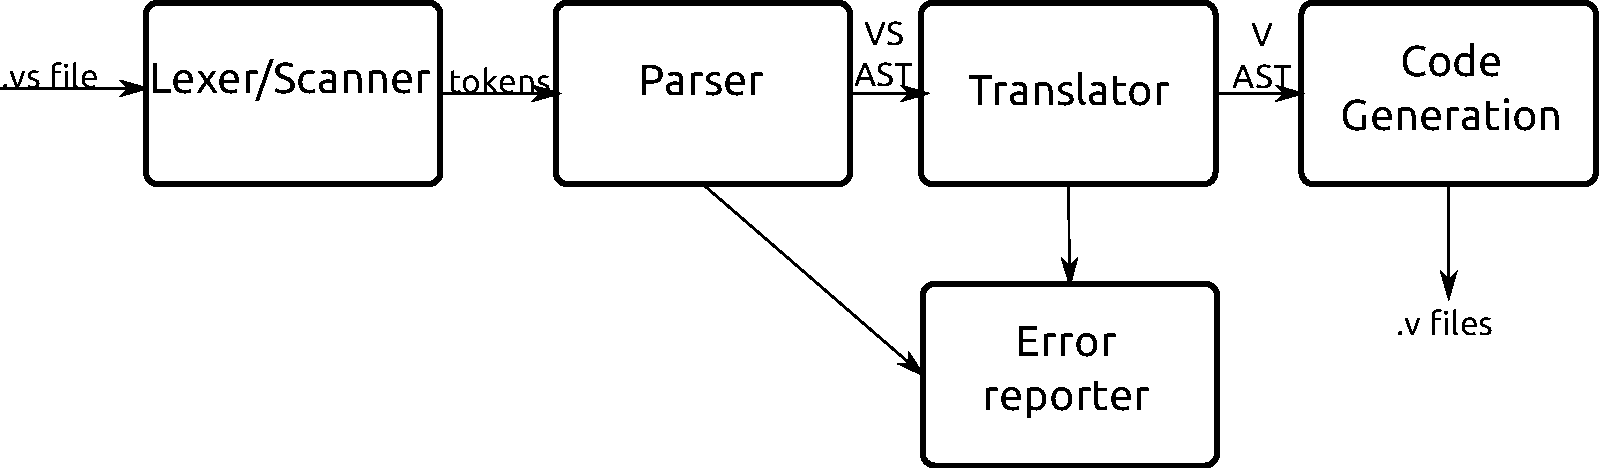
\includegraphics[width=0.7\textwidth]{blockdiagram-inkscape.pdf}\end{center}\end{figure}
    Like any other compiler, Verishort uses a lexer, a parser, and a translator.  The lexer parses the input into tokens.  The parser parses the tokens to generate an abstract syntax tree for Verishort, with position information for future error reporting.  It also checks for syntactical correctness.  Then, the translator creates a new Verilog-friendly syntax tree by translating the original Verishort tree, accounting for semantic correctness and generating all the necessart temporaries.  Finally, the code generator takes the Verilog syntax tree and outputs syntactically correct Verilog code.
    \subsection{Error Recovery}
	Syntactic errors are reported during parsing. The grammar has a few rules designed to catch specific errors, but it is difficult to anticipate them, and unexpected errors are reported immediately.\\ 
	The following code, for example, attempts to anticipate the problem with attaching \texttt{else} blocks to clock edge conditions:\\
	\texttt{IF LPAREN condition\_clock RPAREN stmt ELSE stmt \{ raise (Parse\_Failure(``Clock edge if statements may not have else clauses.'', Parsing.symbol\_start\_pos ())) \}}\\
Semantic errors, such as assignment width mismatches, are reported during translation.  Errors are reported with the input file name, line number, and character position, which is recorded during parsing and passed to the translator in the AST.  The Verishort compiler is fail-fast: once an error is discovered, the compiler reports the error and terminates without attempting to continue compilation.
%%%%%%%%%%%%%%%%%%%%%%%%%%%%%%%%%%%
% TODO: Scott
%%%%%%%%%%%%%%%%%%%%%%%%%%%%%%%%%%%
\section{Testing Plan}
We had two strategies to test our language.  Our first was to build small 33 test cases.  For example, there was a test for implementing multiple modules, a test for block comments, and a test for gating clocks.  Initially, we planned to implement a test bench in Perl using the Posix command \texttt{diff} which would loop through these test cases to compare the output of our compiler with hand-generated expected Verilog code.  This worked until we actually started running the compiler and found minor but crucial differences between the output of the compiler and the generated Verilog code.  The differences did not indicate errors but rather differences in ordering and naming (we began putting an underscore in front of all variable names, for example, to avoid conflicts with Verilog reserved words).  For this reason,  this system was no longer worth maintaining as it was more efficient to manually verify contents due to continued differences in naming and ordering.  However, the Verishort test cases remained useful and we began using them as miniature regression tests to ensure that the compiler was handling output correctly.

Our second strategy was to build small but non-trivial programs and ensure that our compiler translated them into working Verilog and ran them with stim files.  Three of these files were built: helloworld, gcd, and a memoryarray.  These can be run by running 'make helloworld', 'make gcd', 'make memoryarray'.  (These are in the Makefile for the convenience of the tester.)
    
%%%%%%%%%%%%%%%%%%%%%%%%%%%%%%%%%%%
% Mushy stuff that can be done at the end.
%%%%%%%%%%%%%%%%%%%%%%%%%%%%%%%%%%%    
\section{Lessons Learned}
The biggest lesson that (we imagine) is stated every year is to start early, stay ahead, and 
don't wait until the last minute. There was a time crunch at the end, even though we were 
relatively ahead of schedule all semester long. In the end, even when it seems most of the compiler 
is built, there are a lot of loose ends to tie up, and random bugs to squash. Just as you may think 
you are finished, two or three more errors will pop up.\\\\
Concerning Verishort, we realized it was very bad to try to improve on a language that we were not entirely familiar with. We ended up having to rely on Scott, who is taking a design class which required Verilog, for 
every single detail on Verilog. We all knew a bit about the language, but not very specific details 
that needed clarifying every now and then. Had we all known and written Verilog code on a regular 
basis, we wouldn't have had a huge learning curve for language knowledge.  In addition, we should have had a clearer vision for what subset of the Verilog language we were going to implement.\\\\ 
Granted, we had a few weeks shaven off our development time since we switched our project from Natural 
to Verishort, but even then, we should have chosen more carefully in that respect. It was a challenge, 
and the challenge overwhelmed. 
\newpage
        
\section{Codebase}
\subsection{Ast.ml}
\lstinputlisting{ast.ml}
\subsection{Asttoimst.ml}
\lstinputlisting{asttoimst.ml}
\subsection{Imst.ml}
\lstinputlisting{imst.ml}
\subsection{Imsttocode.ml}
\lstinputlisting{imsttocode.ml}
\subsection{Parser.mly}
\lstinputlisting{parser.mly}
\subsection{Scanner.mll}
\lstinputlisting{scanner.mll}

\section{Example files}
\subsection{Gcd.vs}
\lstinputlisting{examples/gcd.vs}
\subsection{Gcd.v}
\lstinputlisting{examples/gcd.v}
\subsection{Stim file for gcd}
\lstinputlisting{examples/gcdstim.v}
\subsection{Helloworld.vs}
\lstinputlisting{examples/helloworld.vs}
\subsection{Helloworld.v}
\lstinputlisting{examples/helloworld.v}
\end{document}
